\documentclass[xetex,mathserif,serif]{beamer}
\usepackage{beamerstyle}

\usetheme{default}

\useoutertheme{miniframes}

\usecolortheme{seahorse}
\useinnertheme{circles}

\beamertemplatenavigationsymbolsempty

\title{Μελέτη και υλοποίηση συστήματος αυτοματισμού για την απομακρυσμένη
παρακολούθηση περιβαλλοντικών συνθηκών}

\author{Θεόδωρος Ελευθέριος \textsc{Πάνου}\\071045\\[0.3cm]
{\scriptsize Επιβλέπουσα καθηγήτρια}\\Ιφιγένεια \textsc{Φουντά}}


\institute[ΤΕΙ Αθήνας]{
    Τεχνολογικό Εκπαιδευτικό Ίδρυμα Αθήνας\\
    Σχολή Τεχνολογικών Εφαρμογών\\
    Τμήμα Πληροφορικής
}
\date{Αθήνα, Νοέμβριος 2014}

\begin{document}


\begin{frame}[plain]
    \titlepage
\end{frame}


\begin{frame}\frametitle
    {Η συσκευή}

    \begin{columns}[t]
    \column{6cm}
        \begin{itemize}
        \item Παρακολούθηση περιβάλλοντος δοχείου
        \item Διασύνδεση μέσω HTTP
        \end{itemize}

    \column{6cm}


        \begin{itemize}
        \item Αισθητήρες προσαρτημένοι σε κινητό εξάρτημα
        \item Αυτοματοποίηση μετρήσεων
        \end{itemize}

    \end{columns}

    \begin{center}
    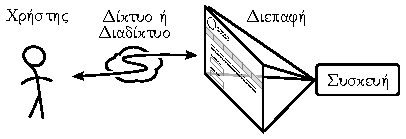
\includegraphics[scale=0.75,clip,viewport=0 -50 151 70]{network_interface-0}
    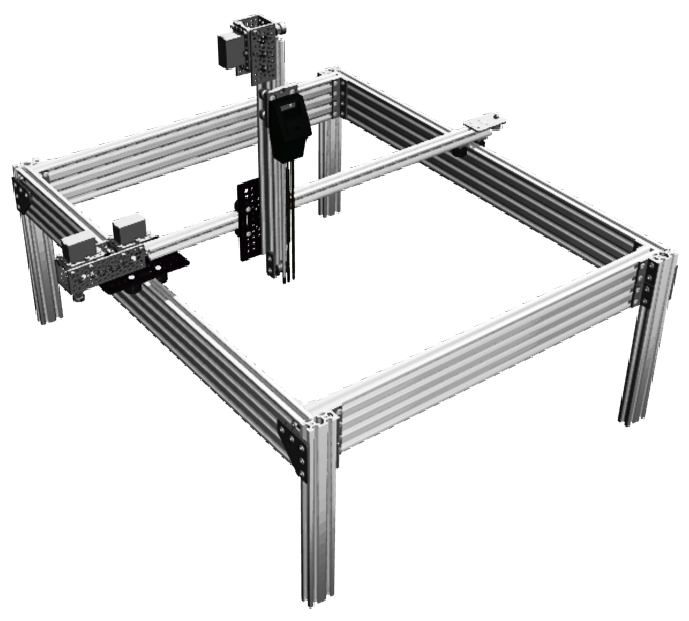
\includegraphics[scale=0.45]{construct_overall}
    \end{center}
\end{frame}


\begin{frame}\frametitle
    {Καθήκοντα συσκευής}

    \begin{columns}[T]
    \column{5.5cm}
    \begin{block}
        {Λήψη δεδομένων HTTP}

        \begin{itemize}
        \item Ενεργοποίηση διακομιστή
        \item Τρόπος διασύνδεσης με τρίτους
        \end{itemize}
    \end{block}

    \column{5.5cm}
    \begin{block}
        {Περιοδική αφύπνιση}

        \begin{itemize}
        \item Έλεγχος χρόνου από πρόσφατη μέτρηση
        \item Εκκίνηση νέου κύκλου εργασιών
        \end{itemize}
    \end{block}
    \end{columns}

    \begin{center}
        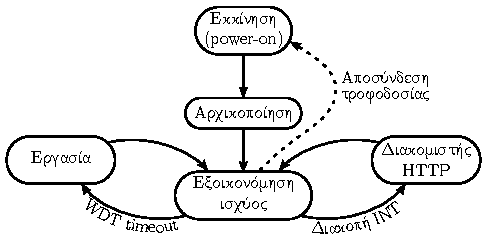
\includegraphics[scale=0.65]{mcu_tasks}
    \end{center}
\end{frame}


\begin{frame}\frametitle
    {Περιβάλλον ανάπτυξης}

    \begin{columns}[t]
        \column{5.5cm}

        \begin{block}
            {Arduino}

            \begin{itemize}
            \item IDE (ανάπτυξη μέσω GUI)
            \item Βιβλιοθήκες
            \item Πλακέτα
            \item Boot Loader
            \item USB σε USART
            \end{itemize}
        \end{block}

        \begin{block}
            {AVR}

            \begin{itemize}
            \item Atmel AVR
            \item Μικροελεγκτής AVR ATmega328
            \item AVR GCC Toolchain
            \end{itemize}
        \end{block}

        \column{6cm}

        \begin{center}
            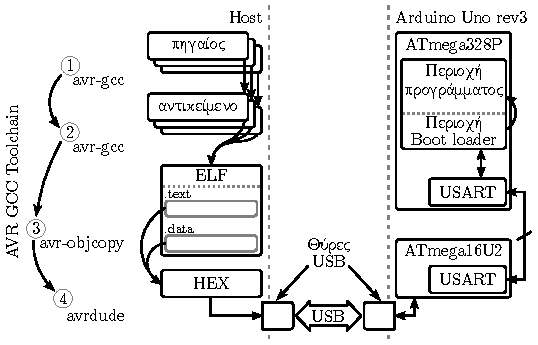
\includegraphics[scale=0.6]{avr_toolchain}\\
            \;
            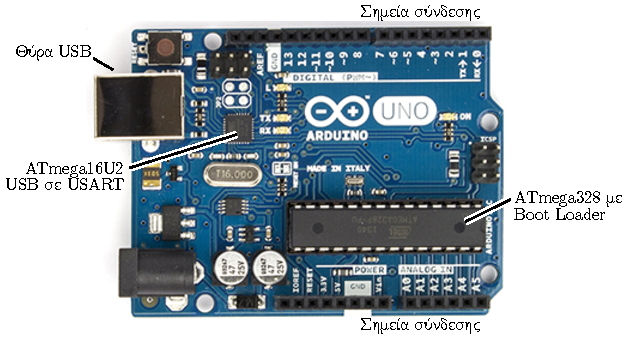
\includegraphics[scale=0.5]{arduino_uno}
        \end{center}
    \end{columns}
\end{frame}


\begin{frame}\frametitle
    {Κεφαλή αισθητήρων}

    \begin{itemize}
    \item Κινητό εξάρτημα με αισθητήρες
    \item Κινείται επάνω και προς το υλικό (3 άξονες γραμμικής)
    \item Επιτρέπει δειγματοληψία σε τυχαία σημεία
    \item Πολλαπλές μετρήσεις παρέχουν μία ιδέα της κατάστασης
    \end{itemize}

    \begin{center}
    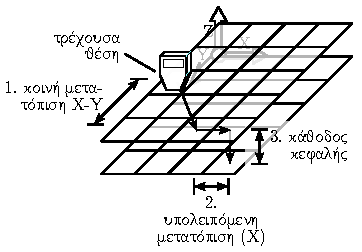
\includegraphics{drive_translation}
    \end{center}
\end{frame}


\begin{frame}\frametitle
    {Υποσύστημα κίνησης}

    \begin{columns}
    \column{5.5cm}
    \begin{itemize}
        \item Έλεγχος θέσης κεφαλής
        \item CPU: διευθέτηση υλικού
        \item Υλικό: Παραγωγή και παύση σήματος ελέγχου
    \end{itemize}

    \column{5.5cm}
    \begin{itemize}
        \item Προφύλαξη από πρόσκρουση στα άκρα
            \begin{itemize}
            \item Επιστροφή και εκ νέου προσπάθεια
            \end{itemize}
    \end{itemize}
    \end{columns}

    \begin{center}
    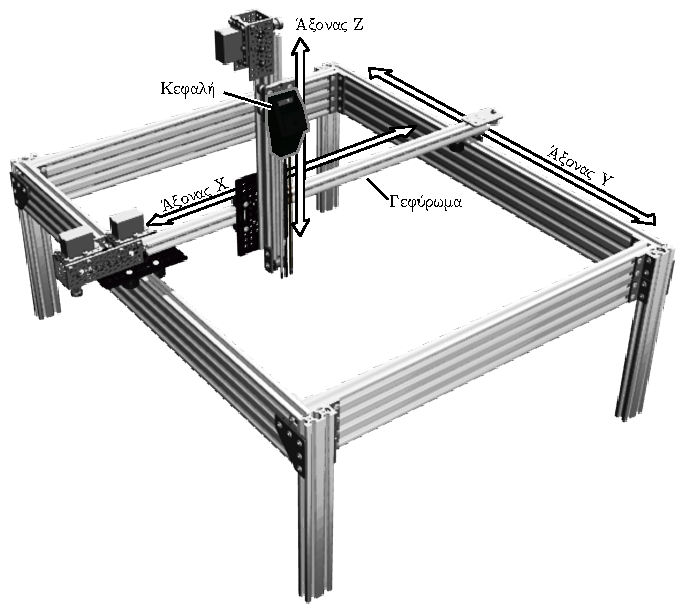
\includegraphics[scale=0.5]{construct_device}
    \end{center}
\end{frame}


\begin{frame}\frametitle
    {Λεπτομέρειες υποσυστήματος κίνησης}

    \begin{columns}[T]
    \column{5cm}
    \begin{itemize}
    \item Υποδιαίρεση επιφάνειας σε διακριτές θέσεις
    \item Σύστημα συντεταγμένων [X, Y, Z]
    \item Παράλληλη μετατόπιση σε επίπεδο X-Y
    \item Θέση επιστροφής (homing) κατά την έναρξη
    \item Προσαρμογή σε ιδεατές διαστάσεις
    \end{itemize}

    \column{6cm}
    \begin{center}
    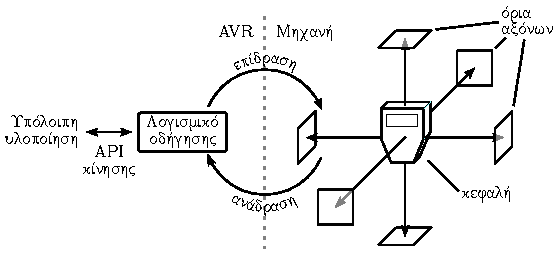
\includegraphics[scale=0.65]{drive_lvl-0}

    \rule{0pt}{0.5cm}

    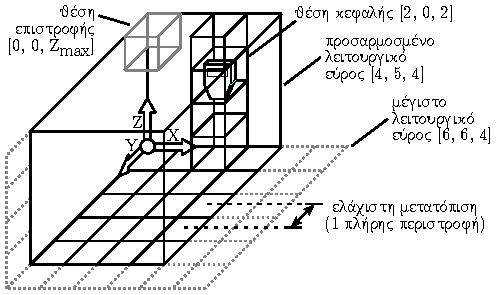
\includegraphics[scale=0.65]{drive_coordinates}
    \end{center}
    \end{columns}
\end{frame}


\begin{frame}\frametitle
    {Κωδικοποιητής κίνησης}

    \begin{columns}[t]
    \column{5.5cm}
    \begin{itemize}
        \item Παρακολούθηση και ενημέρωση σχετικά με περιστροφή
        \item Παραγωγή παλμών από περιστροφή κινητήρα
        \item Προσαυξητικός
    \end{itemize}

    \column{5.5cm}
    \begin{itemize}
        \item Αυτοσχέδιος με χρήση ανακλαστικού αισθητήρα
        \item Ενεργοποιείται μόνο όσο λειτουργεί ο κινητήρας
        \item Ένας για κάθε άξονα κίνησης
    \end{itemize}
    \end{columns}

    \begin{columns}
    \column{5cm}
    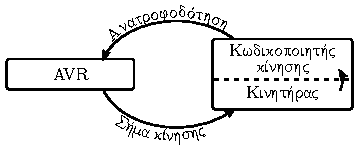
\includegraphics[scale=0.65]{encoder_lvl-0}
    \column{5cm}
    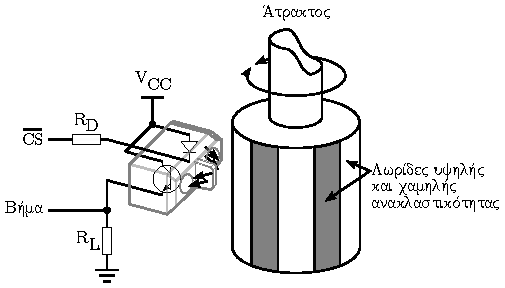
\includegraphics[scale=0.65]{encoder_lvl-1}
    \end{columns}
\end{frame}


\begin{frame}
    \frametitle{Κύκλος μετρήσεων}
    \begin{itemize}
    \item Εκκίνηση ανά σταθερά διαστήματα (κβάντα)
    \item Τυχαία επιλογή θέσεων δειγματοληψίας
    \item Εκτίμηση χρόνου ολοκλήρωσης
    \item Καταχώρηση μετρήσεων
        \begin{itemize}
            \item Ημερ\slash{}ώρα, συντεταγμένες, θερμοκρασία, (RH, pH)
        \end{itemize}
    \end{itemize}

    \rule{0pt}{0.5cm}
    \begin{columns}
    \column{5.5cm}
    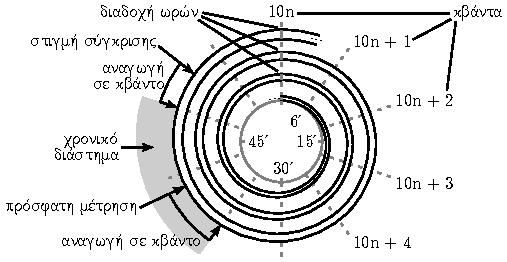
\includegraphics[scale=0.65]{task_interval}

    \column{5.5cm}
    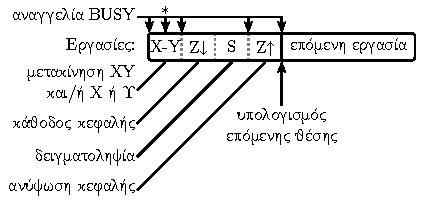
\includegraphics[scale=0.65]{task_estimate-update}
    \end{columns}
\end{frame}


\begin{frame}
    \frametitle{Ημερολόγιο (Log)}
    \begin{itemize}
    \item Διαχείριση εγγραφών μετρήσεων
    \item Διατήρηση πλέον πρόσφατων μετρήσεων
        \begin{itemize}
        \item Κυκλική μνήμη (μείωση επανεγγραφών)
        \item Δυαδική αναζήτηση (μείωση αναγνώσεων)
        \end{itemize}
    \item Εικονικά σετ εγγραφών
        \begin{itemize}
            \item Διευκόλυνση σελιδοποίησης
        \end{itemize}
    \end{itemize}
    \begin{center}
        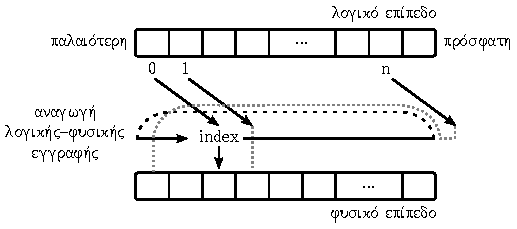
\includegraphics[scale=0.65]{log_structure}
    \end{center}
\end{frame}


\begin{frame}\frametitle
    {Επικοινωνία μέσω HTTP}

    \begin{columns}
    \column{5.5cm}

    \begin{block}{Το HTTP}
        \begin{itemize}
        \item Διάδοση
        \item Πόρος και URI
            \begin{itemize}
            \item \verb~http://example.com~ , \verb~/~
            \end{itemize}
        \item Αναπαράσταση πόρου
        \end{itemize}
    \end{block}

    \begin{block}{Η υλοποίηση}
        \begin{itemize}
        \item Κωδικοί κατάστασης {\tiny (404, 405, 503)}
        \item Πεδία {\tiny (Allow, Retry-After, Transfer-coding)}
        \item Query string, chunked
        \item Αναπαράσταση JSON
        \end{itemize}
    \end{block}

    \column{5.5cm}
    \begin{center}
    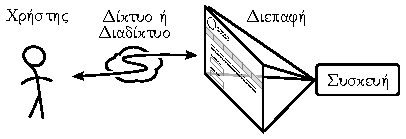
\includegraphics[scale=0.65]{network_interface-0}\\
    \rule{0pt}{1cm}\\
    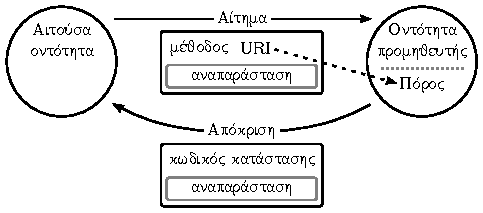
\includegraphics[scale=0.65]{network_requester-provider}
    \end{center}
    \end{columns}
\end{frame}


\begin{frame}\frametitle
    {Ολοκληρωμένο δικτύωσης}

    \begin{itemize}
    \item Υλοποιεί Link, Network, Transport
    \item Λογισμικό οδήγησης του W5100
    \item Υπέρ και κατά διασύνδεσης
    \item Γενικά χαρακτηριστικά (SMD, Socket, διακοπή\slash{}αναγγελία)
    \end{itemize}

    \begin{center}
    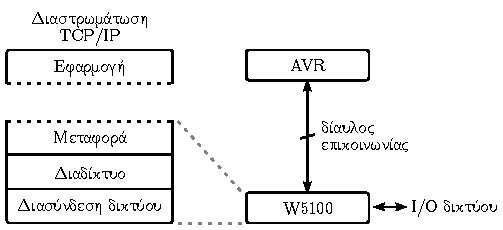
\includegraphics[viewport=0 0 99 110,clip,scale=0.65]{network_lvl-0}
    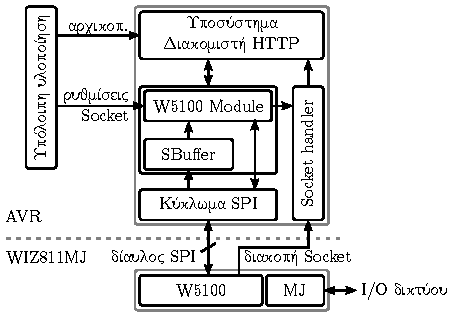
\includegraphics[scale=0.65]{network_lvl-1}
    \end{center}
\end{frame}


\begin{frame}
    {Κύκλος εργασίας μονάδων διακομιστή}

    \begin{center}
    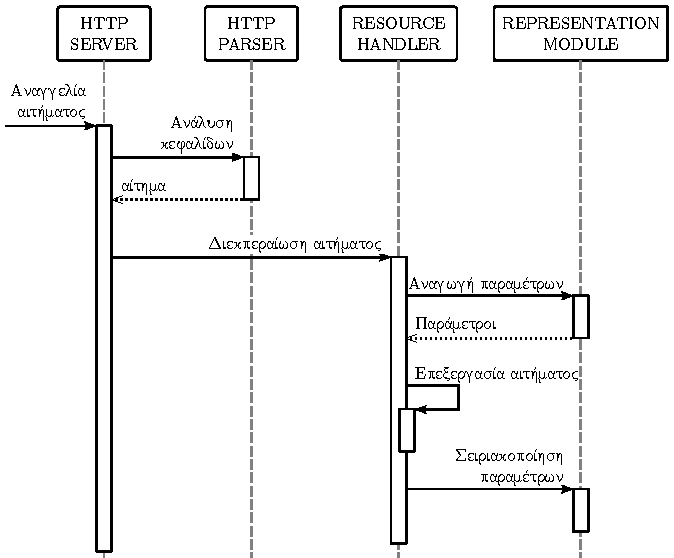
\includegraphics[scale=0.65]{network_server-modules}
    \end{center}
\end{frame}


\begin{frame}\frametitle
    {Πόροι υλοποίησης}

    \begin{center}
    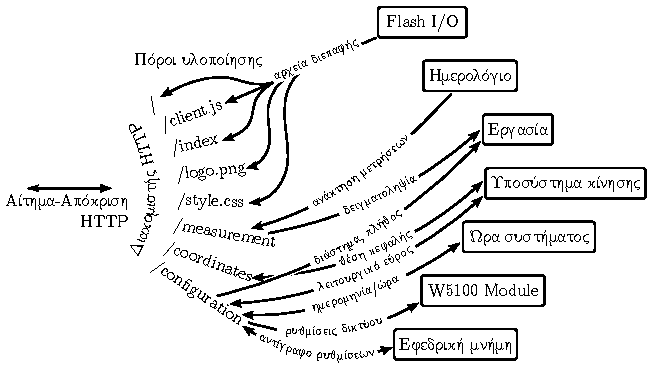
\includegraphics{network_resources}
    \end{center}
\end{frame}


\begin{frame}[plain]
    \begin{center}
    \begin{block}{Ευχαριστώ}
    \end{block}
    \end{center}
\end{frame}


%
% Appendix
%

\begin{frame}[plain]
    \begin{block}
        {Παραρτήματα}
    \end{block}
\end{frame}



\begin{frame}\frametitle
    {Δρομολόγηση και διεκπεραίωση}

    \begin{center}
    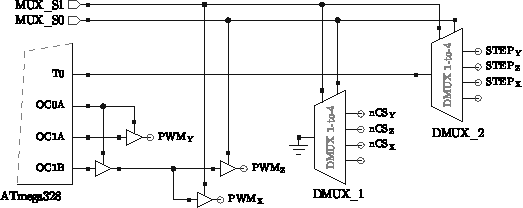
\includegraphics{drive_schem_step-and-pwm}
    \end{center}
\end{frame}


\begin{frame}\frametitle
    {Το υποσύστημα κίνησης συνολικά}

    \begin{center}
    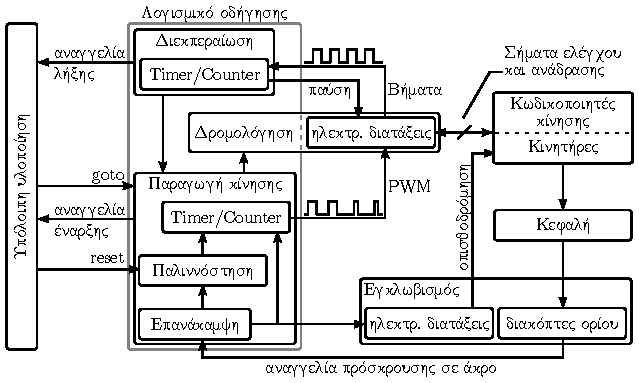
\includegraphics{drive_lvl-1}
    \end{center}
\end{frame}


\begin{frame}\frametitle
    {Διαστρωμάτωση κεντρικών μονάδων S\slash{}W και H\slash{}W}

    \begin{center}
    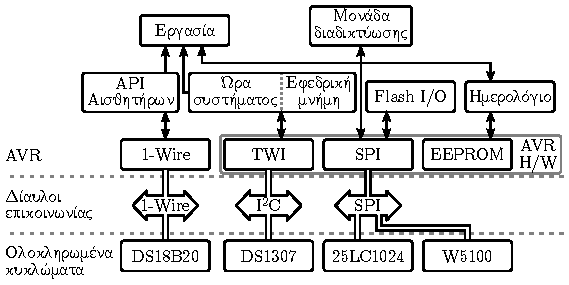
\includegraphics[scale=1]{foundation_lvl-0}
    \end{center}
\end{frame}


\begin{frame}\frametitle
    {Αρχές επεξεργασίας εισερχομένων δεδομένων}

    \begin{columns}[t]
    \column{5cm}
    \begin{itemize}
    \item Ροή χαρακτήρων από Socket {\tiny (next, peek, drop)}
    \item Φίλτρο ανασύνθεσης
    \item Αναγνώριση αναμενόμενων στοιχείων
    \end{itemize}

    \column{6cm}
    \begin{center}
    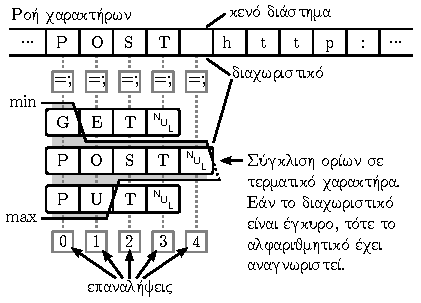
\includegraphics[scale=0.65]{network_stream-match}\\
    \rule{0pt}{0.5cm}\\
    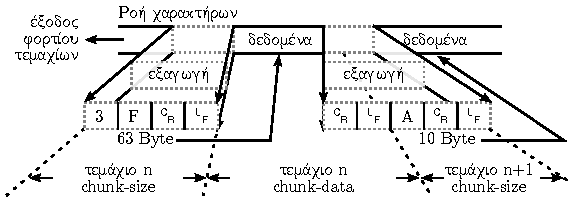
\includegraphics[scale=0.65]{network_chunked-stream}
    \end{center}

    \end{columns}
\end{frame}


\end{document}
